\documentclass[12pt]{article}
\usepackage[russian]{babel}
\usepackage[utf8]{inputenc}
\usepackage[left=2cm, right=2cm, top=2cm, bottom=2cm]{geometry}
\usepackage{amsmath, amsfonts, amssymb, graphicx, cite}

\DeclareMathAlphabet{\mathpzc}{OT1}{pzc}{m}{it}

\title{Цилиндрические маскировочные оболочки с упрощенными свойствами
  материалов видимы}
\author{Min Yan, Zhichao Ruan, and Min Qiu}
\date{4 December 2007}

\begin{document}
\maketitle
\begin{abstract}
  Ранее был предположен способ создания совершенных маскировочных оболочек
  для скрытия объектов от электромагнитного освещения [J. B. Pendry,
    D. Schurig, and D. R. Smith, Science 312, 1780 (2006)]. Однако,
  цилиндрические оболочки, продемонстрированные экспериментально [D. Schurig et
    al., Science 314, 977 (2006)], и предложеные теоретически [W. Cai
    et al., Nat. Photon. 1, 224 (2007)], состоят из материалов с
  упрощенными свойствами для более простой технической реализации, а
  также для избежания бесконечностей в оптических постоянных. Здесь мы
  покажем, что цилиндрические оболочки с упрощенными материальными параметрами
   имеют свойства,
  позволяющие цилиндрическим волнам нулевого порядка проходить через оболочки так,
  как если бы она состояла из однородной изотропной среды, а значит была
  видимой. Для всех цилиндрических волн высшего порядка наши численные
  эксперименты позволяют считать, что упрощенные оболочки наследуют
  некоторые свойства идеальных оболочек, но конечное все же рассеяние
  присутствует.
\end{abstract}

В последнее время наблюдается подъем интереса к реализации
маскировочных оболочек \cite{1, 2, 3, 4, 5, 6, 7, 8}. В частности,
метод замены координат, предложенный в \cite{4}, показывает себя
особенно мощным для создания маскировочных оболочек, которые, в
принципе, могут полностью защищать покрываемые объекты от
электромагнитного (ЭМ) облучения, и в то же время вызывают нулевое
возмущение для внешнего ЭМ поля. В двумерном случае цилиндрическая
оболочка, полученная при помощи такого метода, имеет анизотропные,
зависящие от пространственных переменных оптические постоянные. В
дополнение некоторые параметры материалов имеют бесконечные значения
на внутренней поверхности оболочки. Для облегчения экспериментальной
реализации на микроволновых частотах, Schurig и др. упростили свойства
материалов так, что только один параметр непостоянен, и опущено требование
бесконечности констант для материалов \cite{9}. Авторы отмечают,
что в отличие от идеальных оболочек, упрощенные оболочки сохраняют
свойство огибания потока энергии ценой ненулевого рассеяния на внешней
поверхности раздела. Подобное упрощение для цилиндрических оболочек
также используется в \cite{10}. В этом сообщении мы обеспечим
систематическое теоретическое изучение упрошенных цилиндрических
оболочек. Будет показано, что пустое устройство, построенное при
помощи упрощенной среды не может быть невидимым. В дополнение, устройсвто
не обладает областью в пространстве, абсолютно изолированной от
внешнего мира в электромагнитном плане. Отсюда следует, что совершенная
маскировка при помощи таких упрошенных оболочек невозможна.

Рассмотрим цилиндрическую оболочку с внутренней и внешней границами,
расположенными при $r = a$ и $r = b$ соответственно. Обе среды снаружи
и внутри оболочки заполнены воздухом. Структура, в общем случае,
представляет собой трехслойный цилиндрический рассеиватель. Будем
называть слои, расположенные изнутри к наружи, слоями 1, 2 и 3
соответственно. Наш анализ, подобно всем предыдущим работам, посвящен
нормальному падению. Это значит, что вектор $\mathbf k$
перпендикулярен оси цилиндра. Предпологается, что ЭМ волна
ТЕ-поляризована (т.е. электрическое поле существует только в
направлении оси $z$). Случай ТМ поляризации может быть получен при
помощи замены $E \to -H$, $\varepsilon \to \mu$, и $\mu \to
\varepsilon$. По умолчанию, примем цилиндрические координаты оболочки
за глобальные. В однородных областях пространства (т.е. внутри и
снаружи оболочки) общее решение выражается при помощи функций
Бесселя. Внутри среды заполняющей оболочку, общее волновое уравнение,
описывающее поле $E_z$, может быть записано в виде
\begin{equation}\label{wave}
  \frac{1}{r} \left[\frac{\partial}{\partial r}
    \left(\frac{r}{\mu_\theta} \frac{\partial E_z}{\partial r}
    \right)\right]
  + \frac{1}{r^2} \frac{\partial}{\partial \theta}
  \left(\frac{1}{\mu_r} \frac{\partial E_z}{\partial \theta}\right)
  + k_0^2 \varepsilon_z E_z = 0,
\end{equation}
где $k_0$~--- волновое число в свободном пространстве, $\mu_\theta$, $\mu_r$ и
$\varepsilon_r$~--- профили проницаемости
оболочки, зависящие от поляризации. Зависимость от времени вида $\exp(i
\omega t)$ была использована для вывода уравнения (\ref{wave}).

В идеальном случае, оболочка проектируется так, чтобы сжимать все поля
внутри цилиндрического региона, заполненного воздухом $r < b$, в
цилиндрический кольцевой регион $a < r < b$. Соответствующее
преобразование координат ведет к множеству анизотропных и {\it
изменяющихся в пространстве} параметров материала, заполняющего
оболочку, как описано в \cite{9}. Такой кольцевой цилиндр, конечно,
может обеспечить совершенную маскировку \cite{11}, но требует
бесконечных значений оптических постоянных на внутренней границе
оболочки. Для избежания трудностей в изготовлении оболочек, были использованы
упрощенные параметры \cite{9}. Они имеют следующую форму:
\begin{equation}\label{material}
  \mu_r = \left(\frac{r - a}{r}\right)^2, \quad
  \mu_\theta = 1, \quad
  \varepsilon_z = \left(\frac{b}{b - a}\right)^2.
\end{equation}
Для достижения маскировки от ТМ волн используется тот же набор
параметров, но для величин $\varepsilon_r$, $\varepsilon_\theta$ и
$\mu_z$ \cite{10}. Тем не менее, заметим, что процедура упрощения
параметров материала примененная в \cite{9} довольно спорная, так как
вывод был основан на предположении, что $\mu_\theta$ является
константной. Очевидно, что инвариант $\mu_\theta$ может быть вынесен за
знак дифференциального оператора в \eqref{wave}. Таким образом,
поведение волны внутри маскировочной оболочки изменяется по сравнению с
таковомым в идеальной оболочке.

Поскольку параметры материала в (\ref{material}) азимутально
инвариантны (что также верно для параметров идеальной оболочки), мы
можем использовать разделение переменных $E_z = \Psi(r)
\Theta(\theta)$. Уравнение (\ref{wave}) может быть разложено на два уравнения:
\begin{equation}\label{angle}
  \frac{d^2 \Theta}{d \theta^2} + m^2 \Theta = 0,
\end{equation}
\begin{equation}\label{radius}
  \frac{d}{dr} \left(\frac{r}{\mu_\theta} \frac{d \Psi}{dr}\right)
  + k_0^2 r \varepsilon_z \Psi - m^2 \frac{1}{r \mu_r} \Psi = 0,
\end{equation}
где $m$ целое. Решением (\ref{angle}) является $\exp(i m
\theta)$. Уравнение (\ref{radius}) это однородное дифференциальное
уравнение второго порядка. Ожидается, что оно имеет два независимых
решения. Предположим теперь, что решение уравнения (\ref{radius})
для фиксированного $m$ может быть записано как $\mathpzc A_m Q_m +
\mathpzc B_m R_m$, где $\mathpzc A_m$ и $\mathpzc B_m$~---
постоянные. $Q_m$ и $R_m$~--- функции от $r$. Тогда решения волновых
уравнений в трёх слоях (номер слоя указан в верхнем индексе) могут
быть описаны как
\begin{equation}\label{layer-1}
  E_z^1 = \sum_m \mathpzc A_m^1 J_m(k_0 r) \exp(i m \theta),
\end{equation}
\begin{equation}\label{layer-2}
  E_z^2 = \sum_m \left\{\mathpzc A_m^2 Q_m + \mathpzc B_m^2
  R_m\right\} \exp(i m \theta), 
\end{equation}
\begin{equation}\label{layer-3}
  E_z^3 = \sum_m \left\{\mathpzc A_m^3 J_m(k_0 r) + \mathpzc B_m^3
  H_m^{(2)}(k_0 r)\right\}  \exp(i m \theta),
\end{equation}
$H_m^{(2)}$~--- это функция Ганкеля второго рода, которая отвечает
внешней цилиндрической волне. Слагаемые $J_m$ и $H_m^{(2)}$ в третьем
слое физически отвечают падающей и отраженной волнам соответственно.
Это значит, что задача рассеяния становится задачей нахождения, в
первую очередь, $\mathpzc A_m^1$ (перенесенное поле) и $\mathpzc
B_m^3$ (отраженное поле) при заданных $\mathpzc A_m^3$ \cite{12}.
$\mathpzc A_m^2$ и $\mathpzc B_m^2$ сравнительно менее интересны с
физической точки зрения. Коэффициенты находятся из соотношений для
тангенциальных полей ($E_z$ и $H_\theta$) на границах раздела слоях.
Благодаря ортогональности функции $\exp(i m \theta)$ цилиндрические
волны разных порядков разделяются. Поэтому мы можем исследовать
перенос и рассеяние от оболочи для каждого отдельного порядкового
номера $m$.

Подставив упрощенные параметры материала в (\ref{radius}) получим
\begin{equation}\label{radius-material}
  \left(r - a\right)^2 \frac{d^2 \Psi}{d r^2}
  + \frac{\left(r - a\right)^2}{r} \frac{d \Psi}{d r}
  + \left[\left(r - a\right)^2 \left(\frac{b}{b - a}\right)^2 k_0^2 -
    m^2\right] \Psi
  = 0.
\end{equation}
Уравнение (\ref{radius-material}) имеет две незначительные
сингулярности при $r = 0$ и $r = a$ для $m \ne 0$. Стоит заметить, что
с идеальными параметрами уравнение (\ref{radius}) запишется в свою
очередь как
\begin{equation}\label{radius-ideal}
  \left(r - a\right)^2 \frac{d^2 \Psi}{d r^2}
  + \left(r - a\right) \frac{d \Psi}{d r}
  + \left[\left(r - a\right)^2 \left(\frac{b}{b - a}\right)^2 k_0^2 -
    m^2\right] \Psi
  = 0.
\end{equation}

Для $m = 0$ упростим (\ref{radius-material}) далее до
\begin{equation}\label{radius-material-0}
  r^2 \frac{d^2 \Psi}{d r^2}
  + r \frac{d \Psi}{d r}
  + r^2  k_0^2 \left(\frac{b}{b - a}\right)^2 \Psi
  = 0.
\end{equation}
Это уравнение Бесселя нулевого порядка. Оно также имеет несущественную
сингулярность при $r = 0$. Уравнение (\ref{radius-material-0})
предполагает, что падающая цилиндрическая волна нулевого порядка будет
освещать упрощенную оболочку как однородную изотропную среду с
эффективным индексом рефракции $n_{\mathrm {eff}} = \frac{b}{b - a}$.
Поэтому ее перенос через оболочку определяется эталонным эффектом
конечной среды.

Когда $m \ne 0$, волновые решения определяются из
(\ref{radius-material}). Сравнивая (\ref{radius-material}) и
(\ref{radius-ideal}), увидим, что на радиальных позициях $r \gg a$
(\ref{radius-material}) асимптотически приближается к
(\ref{radius-ideal}), т.к. $r - a \approx r$. Это показывает, что все
цилиндрические волны высших порядков будут иметь схожее поведение в
обоих случаях при $r \gg a$, а также, значит, важность параметра $b$
при котором среда оболочки заканчивается. В дальнейшем, определим
коэффициент рассеяния $s_m$ для каждого порядкового номера
цилиндрической волны $m$. Коэффициент рассеяния для каждого
порядкового номера определяется как $s_m = |\mathpzc B_m^3 / \mathpzc
A_m^3|$. Аналитически получить $s_m$ можно, зная два решения уравнения
(\ref{radius-material}) (напр. $Q_m$ и $R_m$) в явном виде. Однако,
несмотря на внешнюю схожесть, уравнение (\ref{radius-material}) в
отличие от (\ref{radius-ideal}) не решается с помощью аналитического
метода Фробениуса \cite{13}. Здесь, мы решаем задачу при помощи метода
конечных элементов. Поле снаружи оболочки находится численно и затем
используется для нахождения коэффициентов $\mathpzc A_m^3$ и $\mathpzc
B_m^3$ с помощью подгонки. На следующем шаге известен $s_m$. Решения с
разными азимутальными порядками получается вариацией азимутальной
зависимости циркулярного источника внешнего излучения. Задача
отражения численно разрешима, т.к. функционалы $\varepsilon_z
\mu_\theta$ и $\frac{\mu_\theta}{\mu_r}$, входящие в (\ref{radius}), в
отличие от случая идеальной оболочки, конечны и не имеют устранимых
сингулярностей для упрощенной среды. Коммерческое программное
обеспечение COMSOL было использовано для расчетов. В нашем случае, мы
фиксировали $a = 0.1$ м и действующую частоту $f = 2$
ГГц. Эффективность оболочки рассмотрена при увеличении $b$ от $0.2$
м. Похожие параметры также могут быть найдены в \cite{14}.

Коэффициенты рассеяния для различных азимутальных порядков как функции
от $b$ показаны на рис. \ref{pikcha-1}. Как и ожидалось, коэффициент
отражения нулевого порядка достаточно далек от остальных номеров из-за
различия в волновых уравнениях. На самом деле, при $m = 0$ существует
аналитическое решение, т.к. поле в среде, заполняющей оболочку
определяется функциями Бесселя \cite{11}. Отличное согласование между
численными и аналитическими результатами для нулевого порядка
подтверждает валидность и аккуратность нашего подхода. Используя
аналитический подход, мы получили, что коэффициент отражения нулевого
порядка сходится к $0.867$ по отношению к $b$. Несмотря на то, что
индекс эффективности оболочки стремится к 1 с возрастанием $b$, фазовая
вариативность волны нулевого порядка внутри среды оболочки возрастает,
т.к. $k_0 \frac{b}{b - a} (b - a) = k_0 b$. Это объясняет, почему
кэффициент рассеяния сходится к числу, отличному от нуля.
Существование коэффициента рассеяния нулевого порядка не дает оболочке
быть полностью невидимой.

В сравнении с коэффициентом отражения нулевого порядка, коэффициенты
высших порядков (при $m = 1, 2$ показаны на рис. \ref{pikcha-1})
показывают похожее осцилирующее поведение, и, в целом, намного
меньше. Коэффициенты отражения сходятся к числам более близким к $0$ с
увеличением числа $m$. На определенных промежутках для числа $b$
(напр. около $b = 0.225$ м и $m = 1$) измеренное значение $\mathpzc
B_m^3$ меняет знак, и поэтому коэффициент отражения, кажется,
отскакивает от отрицательного значения. Нам следует отметить, что
коэффициенты отражения для высших порядков достаточно малы, что
частично наследуется от идеальных оболочек, основанных на
преобразовании координат \cite{15}. Как бы то ни было, наши расчеты показывают,
что коэффициенты отражения высших порядков не сходятся к нулю, даже
когда стенки оболочки очень толстые.

Помимо необходимости нулевого рассеяния (невидимости), устройство
также должно предоставлять внутренней области полную ЭМ изоляцию от
внешнего мира, чтобы быть маскировочной оболчкой. Поэтому важно знать,
как сильно внешнее ЭМ поле проникает через упрощенную оболочку. Снова,
рассмотрим задачу для каждой компоненты цилиндрической волны отдельно.
Коэффициент переноса, определенный как $t_m = |\mathpzc A_m^1 /
\mathpzc A_m^3|$, используется для описания проникновения поля через
оболочку. При $m = 0$, величина поля, перенесенного внутрь, может быть
измерена аналитически, она показана на рис. \ref{pikcha-2} как функция
от $b$. Наблюдаемый перенос осцилирует и сходится к 1 с увеличением
$b$. Численное решение также это подтверждает. Для $m \ne 0$ рассчеты
МКЭ показывают, что поле за оболочкой близко к нулю. Все коэффициенты
переноса меньше $0.005$, и, поэтому, не показаны на
рис. \ref{pikcha-2}. Это показывает, что контур $r = a$ предоставляет
изоляцию внутренней зоны от внешней, но только для цилиндрических волн
высших порядков. Поэтому все объекты, помещенные за оболочку, видимы
для компоненты нулевого порядка цилиндрической волны. И с другой
стороны, компонента нулевого порядка ЭМ источника, помещенного за
оболочку (или волна, отраженная объектами внутри оболочки),
перенесется наружу. В результате, объекты, покрытые такой упрощенной
оболочкой, будут видимы для внешнего обнаружителя.

Далее, мы численно покажем (используя COMSOL) рассеяние от упрощенной
оболочки падающей плоской волны. Падающая волна распространяется слева
направо и имеет амплитуду $1$. При $b = 0.2$ м, снимок $E_z$, норма
$E_z$, и снимок отраженного $E_z$ изображены на рис. \ref{pikcha-3}
(a1)--(a3) соответственно. Замечено, что амплитуда отраженного поля
составляет примерно половину от падающего поля. Для отраженного поля,
состовляющие Бесселя высших порядков занимают значительную часть.
Напротив, поле за оболочкой, кажется представленным только слагаемым с
функцией Бесселя нулевого порядка. Затем увеличим $b$ до $0.5$ м,
соответсвующие графики показаны на рис. \ref{pikcha-3} (b1)--(b3).
Подобно предыдущему случаю, отраженное поле уменьшено примерно в 2
раза по амплитуде, и теперь представлено в основном слагаемым нулевого
порядка. Норма $E_z$ более однородна вне оболочки, что показывает
лучшую маскировку. Общее уменьшение отражения, как и доминирование
слагаемого нулевого порядка соотносится с полученными коэффициентами
отражения на рис. \ref{pikcha-1}. Когда $b$ увеличено с $0.2$ до $0.5$
м, перенесенное поле в центре оболочки также увеличено по норме от
$0.6032$ до $0.8855$, что также согласуется с рис. \ref{pikcha-2}.

Для полноты, также покажем отражение от оболоки, близкой к идеальной
на рис. \ref{pikcha-3} (c1)--(c3). Параметры материалов оболочки
определяются как $\mu_r = \frac{r - a}{r}$, $\mu_\theta = \frac{r}{r -
  a}$, и $\varepsilon_z = \left(\frac{b}{b - a}\right)^2 \frac{r -
  a}{r}$, при $a = 0.1$ м и $b = 0.5$ м. Чтобы избежать критического
значения на границе при $r = 0.1$ м, мы поместили границу оболочки на
$r = 0.101$ м. В \cite{11} мы подтвердили аналитически, что
эффективность идеальной оболочки крайне чувствительна к положению
внутренней границы. В частности, цилиндрическая волна нулевого порядка
имеет значительное рассеяние и перенос при прохождение через оболочку.
Это подтверждено на рис. \ref{pikcha-3} (c1)--(c3). Отраженное поле
почти полностью представляет собой цилиндрическую волну нулевого
порядка. Даже при таком маленьком изменении положения внутренней
границы, величина поля проникнувшего за оболочку оказывается
значительна, составляя $0.5466$ по норме. Сравнивая (c1)--(c3) и
(b1)--(b3) на рис. \ref{pikcha-3}, мы видим, что упрощенная оболочка
наследует некоторые свойства близкой к идеальной, но в целом
показывает большее отражение, особенно в главной компоненте волны.

В заключение, мы изучили теоретически цилиндрические оболочки с
упрощенными параметрами среды. Такие упрощенные оболочки показывают
свойства, унаследованные от оболочек, полученным с помощью
преобразования координат в уравнениях Максвелла. Тем не менее, ценой
такого упрощения оказывается нечто большее, чем просто ненулевое
рассеяние от поверхности оболочки. Монопольный компонент падающей
волны будет всегда показывать относительно высокое отражение.
Цилиндрические волны высших порядков также показывают отличное от нуля
(хотя меньшее) отражение, даже когда стенка оболочки оказывается очень
толстой, как показано в наших численных экспериментах. Кроме того, что
устройство оказывается видимым само по себе, оно не может полностью
скрыть ЭМ поле, из-за проникновения монопольного компонента. Поэтому,
такая маскировка далека от идеальной. Наконец, поскольку монопольное
поле ведет себя с упрощенной оболочкой, как с прозрачной стеклянной
трубкой, обнаружение любого скрытого объекта может быть легко
осуществлено с помощью источника энергии с максимальной энергией
монопольного компонента.

Работа осуществлена при поддержке Шведской Организации Стратегических
исследований (SSF) через программу INGVAR, Центра Стратегических
Исследований SSF в Фотонике, и Шведского Министерства Исследований
(VR).

\begin{thebibliography}{99}
\bibitem{1} A. Greenleaf, M. Lassas, and G. Uhlmann,
  Physiol. Meas. 24, 413 (2003).

\bibitem{2} A. Alu and N. Engheta, Phys. Rev. E 72, 016623 (2005).

\bibitem{3} U. Leonhardt, Science 312, 1777 (2006).

\bibitem{4} J. B. Pendry, D. Schurig, and D. R. Smith, Science 312,
  1780 (2006).

\bibitem{5} D. A. B. Miller, Opt. Express 14, 12 457 (2006).

\bibitem{6} G. W. Milton, M. Briane, and J. R. Willis, New J. Phys. 8,
  248 (2006).

\bibitem{7} A. Greenleaf, Y. Kurylev, M. Lassas, and G. Uhlmann,
  Commun. Math. Phys. 275, 749 (2007).

\bibitem{8} H. Chen, X. Jiang, and C. T. Chan, arXiv:0707.1126.

\bibitem{9} D. Schurig, J. J. Mock, B. J. Justice, S. A. Cummer,
  J. B. Pendry, A. F. Starr, and D. R. Smith, Science 314, 977 (2006).

\bibitem{10} W. Cai, U. K. Chettiar, A. V. Kildishev, and
  V. M. Shalaev, Nat. Photon. 1, 224 (2007).

\bibitem{11} Z. Ruan, M. Yan, C. W. Neff, and M. Qiu,
  Phys. Rev. Lett. 99, 113903 (2007).

\bibitem{12} For example, the right-traveling incidence plane wave in
  Bessel functions, or a exp jk0 x can be expandedP generalized
  Fourier series, as m i m Jm k0 r exp im. Therefore A3 m can be
  determined beforehand. See D.Felbacq et al., J. Opt. Soc. Am. A 11,
  2526 (1994).

\bibitem{13} G. Arfken, Mathematical Methods for Physicists (Academic,
  New York, 1970), 2nd ed., Chap. 9.

\bibitem{14} S. A. Cummer, B.-I. Popa, D. Schurig, D. R. Smith, and
  J. B. Pendry, Phys. Rev. E 74, 036621 (2006).

\bibitem{15} For comparison purpose, it should be mentioned that the
  scattering coefficient in any order of an annular cylinder
  varies between 0 and 1 as a function of either its refractive
  index (as geometry is fixed) or its outer radius (as material
  and inner radius are fixed).
\end{thebibliography}

\begin{figure}[p]
  \centering
  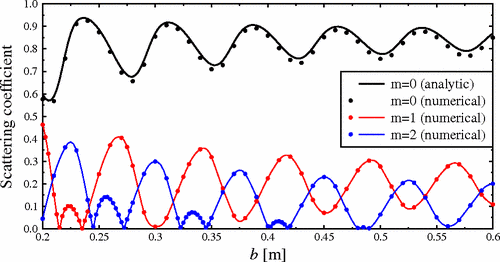
\includegraphics[height=0.12\paperheight]{1.png}
  \caption{}
  \label{pikcha-1}
\end{figure}
\begin{figure}[p]
  \centering
  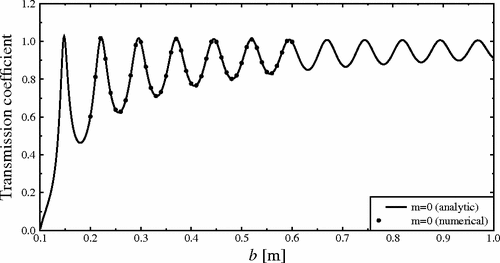
\includegraphics[height=0.12\paperheight]{2.png}
  \caption{}
  \label{pikcha-2}
\end{figure}
\begin{figure}[p]
  \centering
  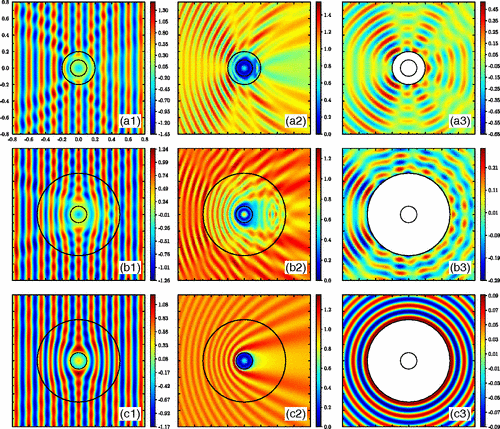
\includegraphics[height=0.3\paperheight]{3.png}
  \caption{}
  \label{pikcha-3}
\end{figure}

\end{document}
